\documentclass{article}
\usepackage{gensymb, amsmath, float, graphicx, epstopdf}
\restylefloat{table}
\usepackage[margin=0.75in]{geometry}
\usepackage{verbatim}
\begin{document}

\title{Ocean Bowl Bootcamp 1: Ocean Currents}
\author{Michael Shen}
\date{October 19, 2014}
\maketitle

\section{Quick Summary}
\begin{itemize}
	\item The Coriolis Effect is the cause of the rotational nature of ocean currents. Each rotational system is called a \textbf{gyre}; there are five major ocean gyres. It's best to memorize that the currents rotate \textbf{clockwise in the Northern Hemisphere} and \textbf{counter-clockwise in the Southern Hemisphere} (Figure 1). This same relationship will hold for other things we will cover in the future.
	\item Currents are measured in \textbf{sverdrup}. One sverdrup = One million $m^3/s$ of water flow. One sverdrup is approximately the total rate of freshwater flow into the oceans, while currents push 50-150 sverdrup. This significant flow rate is why shipping lanes heavily utilize these currents. For example, the \textbf{Gulf Stream} was used to get to Europe from the Americas, while the \textbf{Agulhas Current} effectively blocked Europe from sailing to India around Africa.
	\item Ocean currents are not all surface currents. They move vertically through the water column due to \textbf{thermohaline circulation (THC)} (Figure 2). This is the shorthand for saying that colder and saltier water is denser and thus sinks. Water takes around \textbf{1000 years} to complete one circuit.
	\item The temperature and salt concentration gradients in the ocean waters are also referred to as the \textbf{thermocline} and \textbf{halocline}, respectively (Figure 3). Note the rapid drop in temperature between depths of 0 and 500m. This is because the primary factor in determining ocean water temperature is energy from light. However, light is dispersed very quickly (exponentially) by water. Most of it is absorbed in the first 10m and 99\% of the light is absorbed in the first 200m of the ocean. \textbf{No light penetrates past 1000m}; this is why there is very little temperature drop between 1000 and 7000m. 
\end{itemize}

\section{Figures}
\begin{figure}[H]
    \centering
    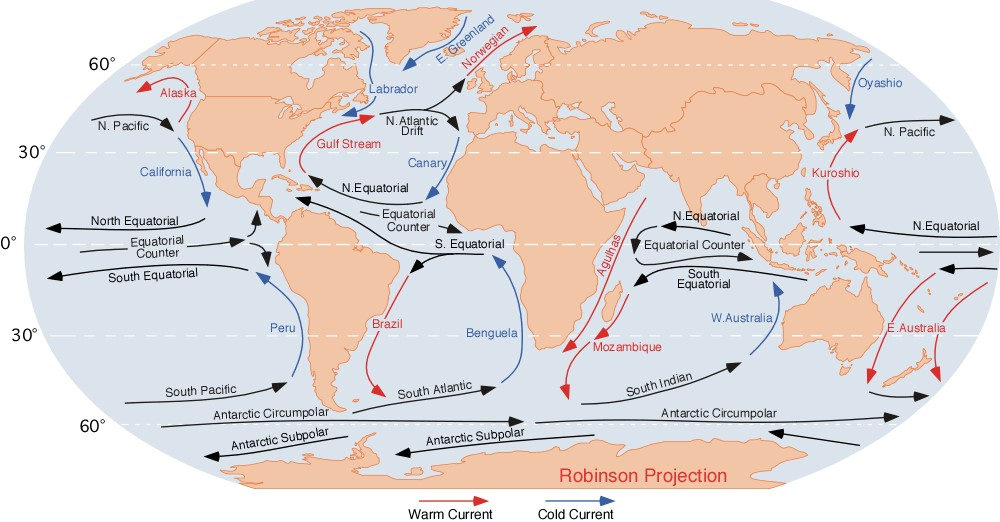
\includegraphics[width=\textwidth]{./Images/BC1_CurrentMap.jpg}
    \caption{Map of all significant ocean currents, memorize them!}
\end{figure}
\begin{figure}[H]
	\centering
	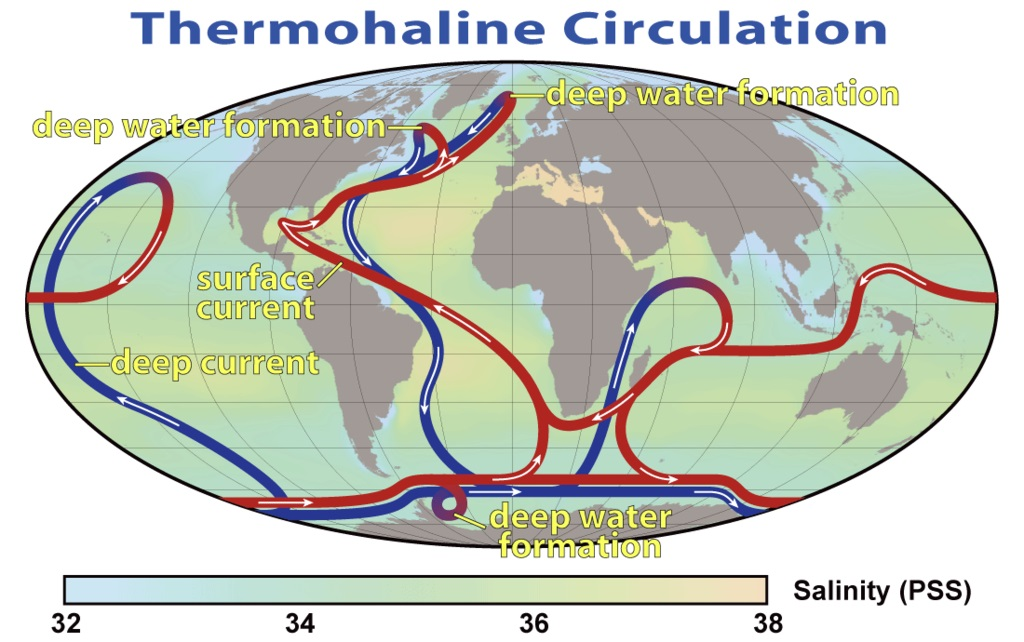
\includegraphics[width=\textwidth]{./Images/BC1_THC.jpg}
	\caption{Diagram of thermohaline circulation in the worlds oceans}
\end{figure}
\begin{figure}[H]
	\centering
	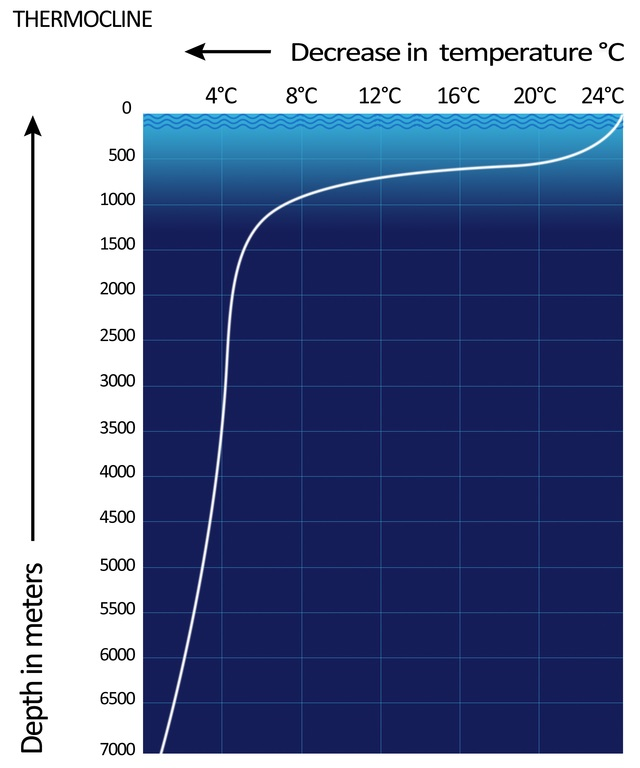
\includegraphics[scale=1]{./Images/BC1_Thermocline.jpg}
	\caption{Graph of an ocean's thermocline. Note the rapid decrease in temperature until 1000m, where temperature change effectively halts because no light penetrates past 1000m.}
\end{figure}

\end{document}